\documentclass[aspectratio=169]{beamer}
\usetheme{Madrid}
\usecolortheme{default}

\usepackage[utf8]{inputenc}
\usepackage{amsmath,amssymb}
\usepackage{booktabs}
\usepackage{tikz}
\usetikzlibrary{arrows.meta,positioning}

\definecolor{deepblue}{RGB}{25,87,140}
\definecolor{warmred}{RGB}{190,70,55}
\setbeamercolor{structure}{fg=deepblue}
\setbeamertemplate{navigation symbols}{}

\title[Shallow-water project]{A short shallow-water project}
\subtitle{From a physical question to a controlled numerical experiment}
\author{F. Roquet}
\date{\today}

\newcommand{\unit}[1]{\,\mathrm{#1}}

\begin{document}

\begin{frame}
  \titlepage
\end{frame}

\begin{frame}{The aim: one small experiment, one clear result}
  Work in groups of two to investigate a question of your choice with
  the shallow-water model.
  \begin{block}{Keep the scope deliberately small}
    Run a baseline and at least one controlled variation. Change one main
    factor and support your conclusion with a quantitative diagnostic.
  \end{block}
  \begin{itemize}
    \item Start with an assumption based on a physical process.
    \item Use two or three well-chosen cases; more simulations are not the goal.
    \item An animation can reveal a pattern, but it is not sufficient evidence.
  \end{itemize}
  \begin{alertblock}{Model scope}
    The domain remains fully wet: this is not a model of run-up, inundation,
    breaking, or coastal damage.
  \end{alertblock}
\end{frame}

\begin{frame}{Choose a control that matches your question}
  \begin{center}
  \begin{tabular}{p{0.22\textwidth}p{0.68\textwidth}}
    \toprule
    \textbf{Category} & \textbf{Examples of controls} \\
    \midrule
    Initial state & amplitude, radius, position, pulse shape \\
    Bottom depth & uniform depth, shelf depth or width, ridge, input map \\
    Wind forcing & stress, direction, duration, spatial pattern \\
    Domain and grid & $L_x$, $L_y$, aspect ratio, $N_x$, $N_y$ \\
    Rotation & constant Coriolis parameter $f$ \\
    Dissipation & Rayleigh damping timescale \\
    \bottomrule
  \end{tabular}
  \end{center}
  \vfill
  Domain size and resolution are different controls: changing $L_x$ at fixed
  $N_x$ also changes $\Delta x$.
\end{frame}

\begin{frame}{Turn the question into a controlled comparison}
  \centering
  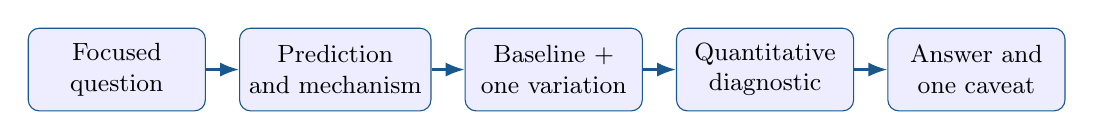
\begin{tikzpicture}[
      node distance=0.42cm,
      box/.style={draw=deepblue, rounded corners, fill=blue!7,
                  minimum width=2.25cm, minimum height=1.05cm,
                  align=center, font=\small},
      arrow/.style={-{Latex[length=2.4mm]}, thick, deepblue}
    ]
    \node[box] (question) {Focused\\question};
    \node[box, right=of question] (prediction) {Prediction\\and mechanism};
    \node[box, right=of prediction] (cases) {Baseline $+$\\one variation};
    \node[box, right=of cases] (measure) {Quantitative\\diagnostic};
    \node[box, right=of measure] (answer) {Answer and\\one caveat};
    \draw[arrow] (question) -- (prediction);
    \draw[arrow] (prediction) -- (cases);
    \draw[arrow] (cases) -- (measure);
    \draw[arrow] (measure) -- (answer);
  \end{tikzpicture}

  \vspace{0.65cm}
  \begin{exampleblock}{Example}
    How does wind duration affect eastern-wall setup? Compare identical 3-hour
    and 6-hour events, then measure the maximum mean surface elevation in the
    four easternmost cells.
  \end{exampleblock}
  \begin{itemize}
    \item Keep all relevant settings fixed except the chosen control.
    \item Record grid spacing, timestep, duration, units, and case parameters.
  \end{itemize}
\end{frame}

\begin{frame}{Workflow, submission, and assessment}
  \begin{columns}[T]
    \column{0.47\textwidth}
      \begin{block}{Use the available time}
        \begin{itemize}
          \item \textbf{Toolbox demonstration:} inspect setup recipes and choose
                a feasible direction.
          \item \textbf{Project block 1:} agree on the question and diagnostic;
                run the baseline and first variation.
          \item \textbf{Project block 2:} analyse, interpret, peer-review, and
                run the whole report notebook again.
        \end{itemize}
      \end{block}
    \column{0.49\textwidth}
      \begin{block}{Submit one executed notebook}
        Start from \texttt{project\_report\_template.ipynb}, rename it
        with your group identifier, and keep the evidence visible.
      \end{block}
      \begin{alertblock}{Assessment: G or U}
        A passing report has a focused question and hypothesis, a controlled
        comparison, quantitative evidence, a physical interpretation, one
        relevant caveat, reproducible settings, and a contribution statement.
        There are no points or weighted criteria.
      \end{alertblock}
  \end{columns}
\end{frame}

\end{document}
